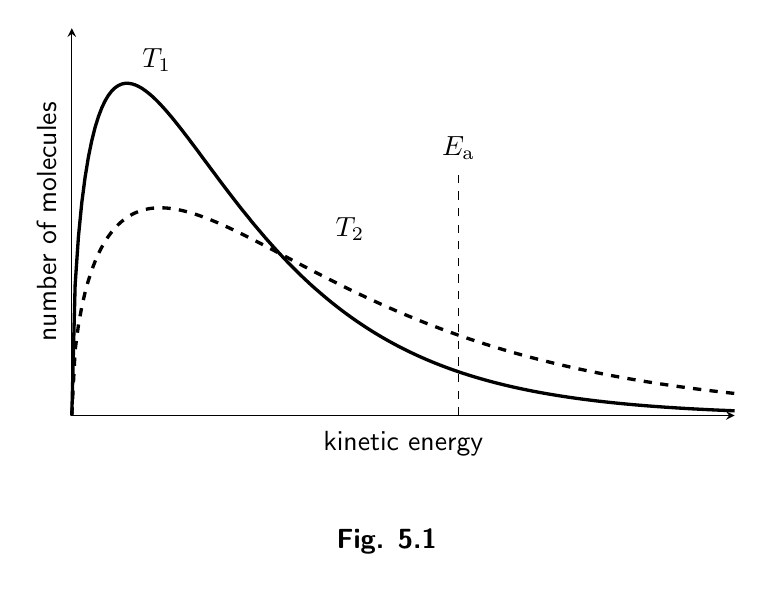
\begin{tikzpicture}[font=\sffamily]
  \begin{axis}[
    width=10cm, height=6.5cm, clip=false,
    axis lines=left, xmin=0, xmax=6, ymin=0, ymax=1.1,
    xtick=\empty, ytick=\empty,
    xlabel={kinetic energy}, ylabel={number of molecules},
  ]
    \addplot[very thick, domain=0:6, samples=200] {2.2*sqrt(x)*exp(-x)};
    \addplot[very thick, dashed, domain=0:6, samples=200] {2.2*1.6^(-1.5)*sqrt(x)*exp(-x/1.6)};
    \draw[dashed] (axis cs:3.5,0)--(axis cs:3.5,0.7) node[above] {$E_\mathrm{a}$};
    \node[above right] at (axis cs:0.55,0.95) {$T_1$};
    \node[above right] at (axis cs:2.3,0.47) {$T_2$};
  \end{axis}
  \node[font=\sffamily\bfseries] at (4,-1.6) {Fig. 5.1};
\end{tikzpicture}
